\clearpage
{\bfseries SRSTI 52-77; 003.11}

\section{EXPLORING THE USE OF ELECTRONIC MEDICAL RECORDS FOR PATIENTS}
\begin{center}
{\bfseries G.Z.Ziyatbekova\textsuperscript{1,2*}, M.K.
Omirzak\textsuperscript{2}, G.Z. P.Kisala\textsuperscript{3}}

\textsuperscript{1}RSE Institute of Information and Computational
Technologies MSHE RK CS, Almaty, Kazakhstan,

\textsuperscript{2}Al-Farabi Kazakh National University, Almaty,
Kazakhstan,

\textsuperscript{3} Lublin Technical University,
Poland,

e-mail: ziyatbekova@mail.ru
\end{center}

The article is devoted to the study of the
information system of electronic medical records of patients in order to
improve the work of the ambulance service. Scientific research in the
field of medicine is given. This article discusses medical information
systems and the principles of their functioning. It also shows the
process of effective work due to medical information system. A
user-friendly interface is used. The following functions are touched
upon: elimination of paperwork, transition to electronic system,
additional medical services. All available methods are presented, which
are the key factors in optimizing all medical processes. Also considered
options for modeling and system development, taking into account all the
relevant issues of automation of medical information systems. The
developed information complex can be used both in polyclinics and in
pharmacies, as well as individually for patients. The article deals with
the study of electronic medical records system. In this work developed a
medical information system and ER system as an application. The
possibility of processing, storing and conveniently viewing the created
data system is provided.

{\bfseries Key words:} ambulance, electronic medical record, medicine,
medicine, website.

\begin{center}
{\large\bfseries ПАЦИЕНТТЕРДІҢ ЭЛЕКТРОНДЫ МЕДИЦИНАЛЫҚ ЖАЗБАЛАРЫН}

\vspace{1em}
{\bfseries ҚОЛДАНУ МҮМКІНДІКТЕРІН ЗЕРТТЕУ}

{\bfseries Г.З.Зиятбекова\textsuperscript{1,2*},
P.Kisala\textsuperscript{3}, М.Қ.Өмірзақ\textsuperscript{2}}

\textsuperscript{1}Қазақстан Республикасы Ғылым және жоғары білім
министрлігі Ақпараттық және есептеуіш технологиялар институты, Алматы,
Қазақстан,

\textsuperscript{2}әл-Фараби атындағы Қазақ ұлттық университеті, Алматы, Қазақстан,

\textsuperscript{3}Люблин техникалық yниверситеті, Польша,

e-mail: ziyatbekova@mail.ru
\end{center}

Мақала жедел жәрдем жұмысын жақсарту мақсатында
пациенттердің электрондық медициналық картасын жүргізудің ақпараттық
жүйесін зерттеуге арналған. Медицина саласындағы ғылыми зерттеулер
келтірілген. Бұл мақалада медициналық ақпараттық жүйелер және олардың
жұмыс істеу принциптері қарастырылады. Медициналық ақпараттық жүйенің
арқасында тиімді жұмыс процесі де көрсетілген. Пайдаланушыға ыңғайлы
интерфейс қолданылды. Келесі функциялар қозғалады: қағазбастылықты жою,
электрондық жүйеге көшу, қосымша медициналық қызметтер. Қазіргі уақытта
барлық медициналық процестерді оңтайландырудың негізгі факторлары болып
табылатын барлық қол жетімді әдістер ұсынылған. Сондай-ақ, медициналық
ақпараттық жүйелерді автоматтандырудың барлық өзекті мәселелерін ескере
отырып, жүйені модельдеу және әзірлеу нұсқалары қарастырылған. Әзірленіп
жатқан ақпараттық кешенді емханаларда да, дәріханаларда да, пациенттер
үшін де жеке пайдалануға болады. Мақалада электронды медициналық
жазбалар жүйесін зерттеу қарастырылады. Бұл жұмыста қосымша ретінде
медициналық ақпараттық жүйе және жедел жәрдем жүйесі жасалды. Құрылған
деректер жүйесін өңдеу, сақтау және ыңғайлы қарау мүмкіндігі
қарастырылған.

{\bfseries Түйін сөздер:} жедел жәрдем, электронды медициналық жазба,
медицина, дәрі-дәрмек, веб-сайт.

\begin{center}
{\large\bfseries ИССЛЕДОВАНИЕ ВОЗМОЖНОСТЕЙ ИСПОЛЬЗОВАНИЯ ЭЛЕКТРОННЫХ МЕДИЦИНСКИХ
КАРТ ПАЦИЕНТОВ}

\vspace{1em}
{\bfseries Г.З. Зиятбекова\textsuperscript{1,2*},
P.Kisala\textsuperscript{3}, М.Қ. Өмірзақ\textsuperscript{2}}

\textsuperscript{1}Институт информационных и вычислительных технологий
КН МНВО РК, Алматы, Казахстан,

\textsuperscript{2}Казахский национальный университет имени аль-Фараби,
Алматы, Казахстан,

\textsuperscript{3}Люблинский технический yниверситет, Польша

e-mail: ziyatbekova@mail.ru
\end{center}

Статья посвящена изучению информационной системы
ведения электронной медицинской карты пациентов с целью улучшения работы
скорой помощи. Приведены научные исследования в области медицины. В
данной статье рассматриваются медицинские информационные системы и
принципы их функционирования. Также показан процесс эффективной работы
благодаря медицинской информационной системе. Использован удобный
интерфейс. Затрагиваются следующие функции: устранение бумажной
волокиты, переход на электронную систему, дополнительные медицинские
услуги. В настоящее время представлены все доступные методы, которые
являются ключевыми факторами оптимизации всех медицинских процессов.
Также рассмотрены варианты моделирования и разработки системы с учетом
всех актуальных вопросов автоматизации медицинских информационных
систем. Разрабатываемый информационный комплекс можно использовать как в
поликлиниках, так и в аптеках, а также индивидуально для пациентов. В
статье рассматривается исследование системы электронных медицинских
карт. В данной работе разработана медицинская информационная система и
система Скорой помощи в качестве приложения. Предусмотрена возможность
обработки, хранения и удобного просмотра созданной системы данных.

{\bfseries Ключевые слова:} скорая помощь, электронная медицинская карта,
медицина, лекарства, веб-сайт.

\begin{multicols}{2}
{\bfseries Introduction.} There are many automated control systems designed
to automate the work of emergency stations and departments, but they are
mostly expensive tools and require expensive equipment and skilled
professionals. This raises the challenge of creating an automated
workstation for an ambulance dispatcher "ambulance". In recent years,
not only has the number of computer equipment in medical institutions
increased, but also the quality of communication has improved
significantly, allowing the system to move to a web-based platform. The
complexity of managing and maintaining the current version of the system
does not allow it to be used in small, private and remote medical
institutions, which makes it difficult to automate the exchange of
information. The transition to the Web platform will allow to expand the
range of medical organizations and implement the system {[}1{]}.

Theoretical methods and research analysis were developed as a research
method. Theoretical methods of research allow you to systematize
information, reveal the nature of various phenomena and objects, to
identify relationships between processes. 7 main problems and 7
principles of their solution:

1.The lack of the principle of normative regulation and incentives to
conduct EMC.

2.Problems and principles of integrated document management in medicine.

3. legal significance

4. ensuring of reliability and rules of collective work

5. defining the right of access to electronic medical document

6. structuring and standardization of medical information for electronic
exchange of medical documents

7. principle of systematic sufficiency

According to electronic medical records management, when developing new
rules, they should include balanced requirements for technical means
used in combination with carefully considered organizational measures.

Development of a web application for the ambulance medical information
system, which allows to automate the work of an ambulance dispatcher in
private and remote municipal health care facilities with the ability to
work remotely. It is designed to increase the productivity of ambulance
workers and reduce processing and data entry time. It also provides
various opportunities for immediate contact with ambulance staff.

{\bfseries Materials and methods.} The general system and the medical
laboratory information system can be integrated with modern medical
equipment. In addition, medical IS make it possible to promptly bring
general statistics about the state of health of the population to
municipal authorities and other state institutions. In this connection,
the electronic medical record is used.

The main goals of the electronic medical record:

\begin{itemize}
\item
  To collect and store electronically as much information as possible
  about a specific person\textquotesingle s health;
\item
  Promptly provide access to this information to authorized medical
  workers, the individual himself and his authorized representatives in
  the most convenient and accessible form for a particular user;
\item
  Creation of specialized electronic services based on this information,
  aimed at medical personnel, at the individual himself, and providing
  improved safety and quality of medical care, as well as improved
  quality of life and health of citizens {[}2{]}.
\end{itemize}

These software packages offer the optimal solution for preparing
reporting documents and, in the opinion of many users, are a necessary
component of any ambulance station. But not every ambulance station
allows for the implementation and maintenance of these software
packages. As before, the main problem of widespread implementation of
these systems and their analogues remains the limitation of financial
availability of these programs at the municipal level.

The next step is to describe the Web technologies for creating an
electronic medical record information system for patients. The
server-side programming language for Web applications is Python. Python
is an interpreted, interactive, object-oriented programming language. It
is created in the django framework to create web applications with
little code. A database is used to systematically store an array of data
collected and easily accessible by an authorized user. It is stored to
retrieve the necessary data from the database as needed. Therefore, the
database was implemented using a SQLite database. The client part and
GUI were implemented using JavaScript language, which allows for a
user-friendly and responsive interface. This allows users to access and
interact with basic data in the database. These actions can range from
simple data querying to defining database schemas that radically affect
the database structure.

{\bfseries Results and discussion.} According to electronic medical
records, when new regulations are developed, they must include balanced
requirements for the technical means used, combined with carefully
considered organizational measures (Fig. 1).

\end{multicols}

\begin{figure}[H]
  \centering
  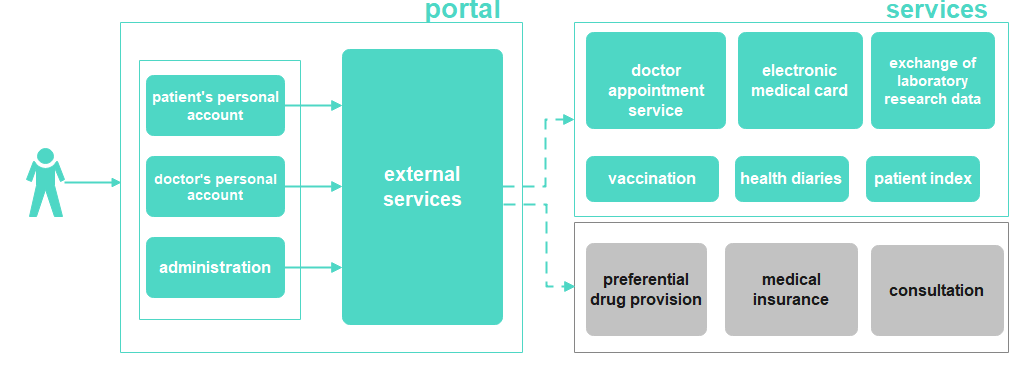
\includegraphics[width=0.8\textwidth]{image15}
  \caption*{Figure 1 - Vision for the medical center portal}
\end{figure}

\begin{multicols}{2}

Information system for electronic medical records of patients before
compiling the technical part of the web-application, it is necessary to
define the requirements to the web-application.

The following requirements apply to a web-based information system for
maintaining electronic medical records:

\begin{itemize}
\item
  Patients must be able to provide complete information;
\item
  Patients should be able to register and then log in to the system;
\item
  information about the patient, records of doctor\textquotesingle s
  visits should always be available in the personal account;
\item
  the doctor must be able to see the patient\textquotesingle s medical
  history, to make records in the medical history;
\item
  the administrator of the web application must be able to view,
  customize information about patients and doctors and arrange for the
  patient to contact the doctor.
\item
  the administrator and physicians need to have separate registration
  and login pages.
\end{itemize}

\end{multicols}

\begin{figure}[H]
  \centering
  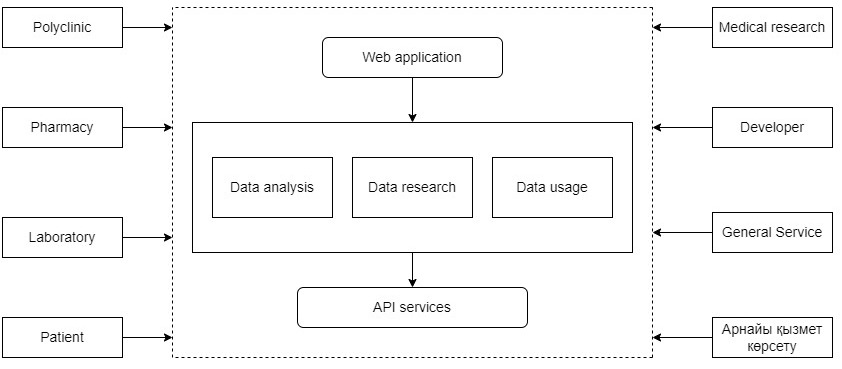
\includegraphics[width=0.8\textwidth]{image16}
  \caption*{Figure 2 - Medical Web Application Connection Diagram}
\end{figure}

\begin{multicols}{2}

The web-based patient application contains an electronic health record,
as described in the previous electronic health record in addition to
including other types of services(Fig. 2). This system establishes
communication with institutions that have access to internal data.
Through the outpatient clinic, pharmacy, and laboratory, certificates
issued by the doctor are indicated. The service and medical research
departments also have the ability to obtain the necessary data
{[}3-4{]}.

Each patient has a unique opportunity to receive the following
information:

\begin{itemize}
\item
  Information about the prescription written by the attending physician;
\item
  Vaccination schedule;
\item
  Information about pharmacies that provide free medications;
\item
  diagnoses;
\item
  hospitalization records.
\end{itemize}

The information received cannot be processed. For visitors to the
e-Health Passport, only training mode is available.

\end{multicols}

\begin{figure}[H]
  \centering
  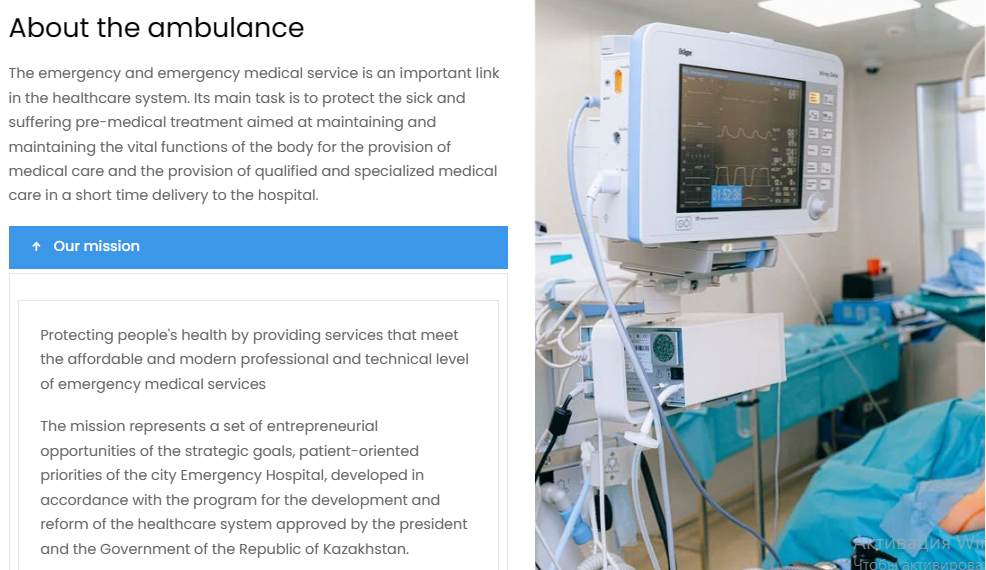
\includegraphics[width=0.8\textwidth]{image17}
  \caption*{Figure 3 - "About the ambulance"}
\end{figure}

\begin{multicols}{2}

Under the ambulance data, we can see our mission, the staff. If we click
on it, we can see information about it (Fig. 3).

The ambulance is an emergency medical service. Therefore, the emergency
medical service is of great importance in the health care system. Its
mission is to protect people\textquotesingle s health by providing
services that are affordable and meet the current professional and
technical level of emergency medical care.

Types of service we provide:

\begin{itemize}
\item
  diagnosis and emergency care;
\item
  Doctors who are invited to come to the home;
\item
  full supervision.
\end{itemize}

For more information, click on the button to see the types of services.
Long-term hospital care provides long-term care measures for patients
who are in serious condition. Specialized care is provided with full
monitoring of patients in need of medical care. Along with sleepwalking,
each place of care was also fully monitored by medical transport
{[}5-6{]}.

Providing first aid to patients in need of emergency care, through a set
of diagnostic and emergency services of a comprehensive type for those
who are referred. Median locations through house call physicians are for
regular patients in certain rural areas and patients who must be checked
regularly over a period of time {[}7-8{]}.

\centering
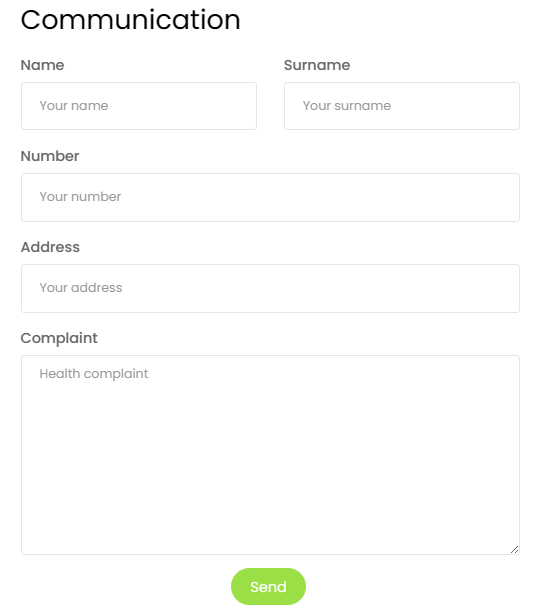
\includegraphics[width=0.8\linewidth]{image18}
\captionof*{figure}{Figure 4 - Emergency communication menu}

In the event of a specific emergency, by visiting the site, you can go
to the emergency communication menu and drop off an application (Fig.
4). The following form is required to be filled out in full.They:

\begin{itemize}
\item
  first name;
\item
  your last name;
\item
  your phone number;
\item
  letter.
\end{itemize}

\end{multicols}

\begin{figure}[H]
  \centering
  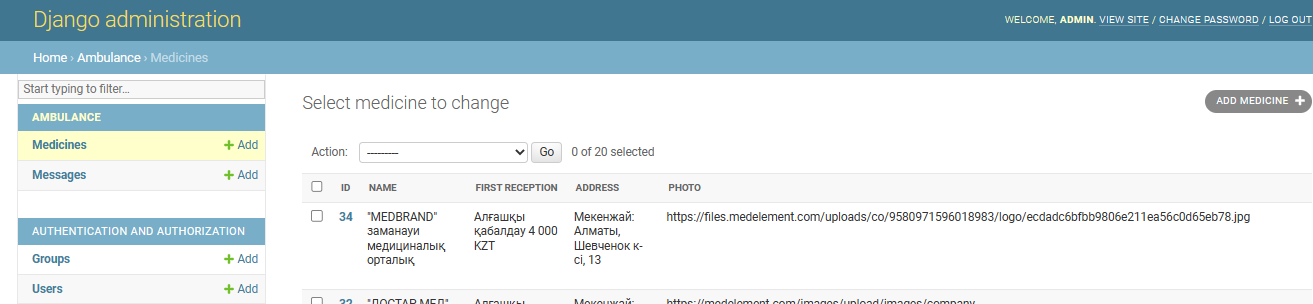
\includegraphics[width=0.8\textwidth]{image19}
  \caption*{Figure 5 - Representation of saving in the database}
\end{figure}

\begin{figure}[H]
  \centering
  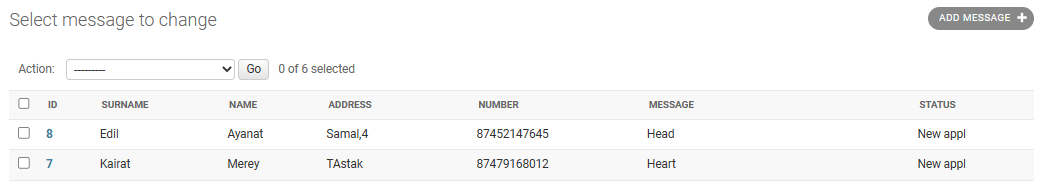
\includegraphics[width=0.8\textwidth]{image20}
  \caption*{Figure 6 - Storing in the database}
\end{figure}

The completed emergency form goes into the database.

\begin{figure}[H]
  \centering
  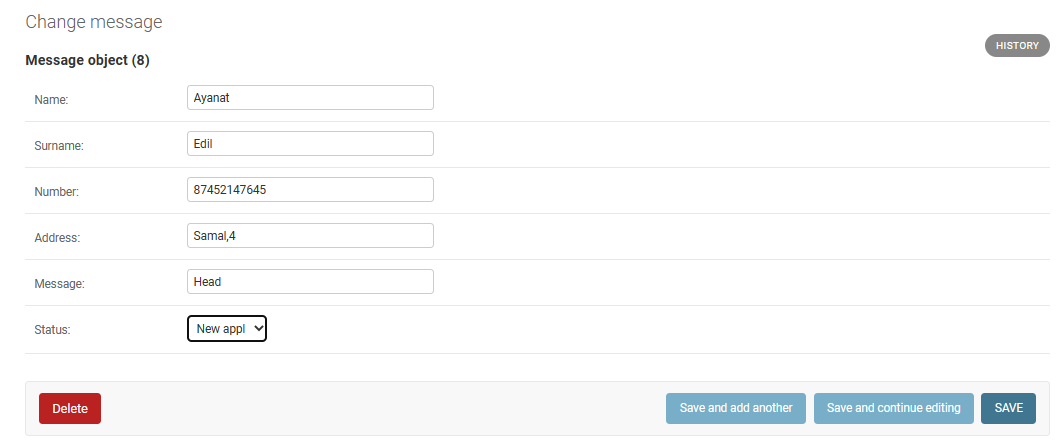
\includegraphics[width=0.8\textwidth]{image21}
  \caption*{Figure 7 - Changing the status in the database}
\end{figure}

\begin{multicols}{2}

You can change the status of incoming data in the database. Also saves
again, changing the status(Fig. 5-6).

You can change the status in the data. The status consists of:

\begin{itemize}
\item
  new request;
\item
  sent;
\item
  completed;
\item
  invalid application.
\end{itemize}

For example, highlight the status "sent" and click the "Save" button. At
this point, the status of the data sent to the database changes (Fig.
8).

\end{multicols}

\begin{figure}[H]
  \centering
  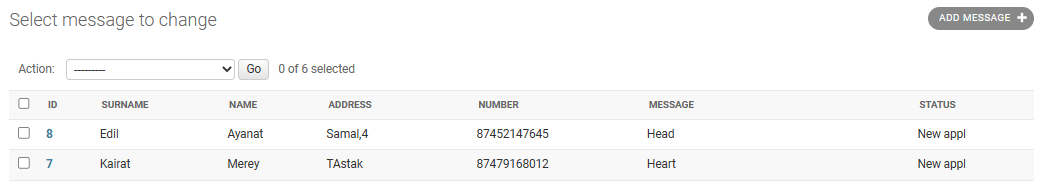
\includegraphics[width=0.8\textwidth]{image20}
  \caption*{Figure 8 - Database when changing and saving the status}
\end{figure}

\begin{multicols}{2}

The results of the study show that the web application, working through
a medical information system, has the ability to communicate with
patients. As a result of the work the following results were achieved:

- Subject area analysis and problem statement;

- analysis of existing software for the automation of emergency medical
care;

- definition of requirements to the developed software.

The sent protocol is processed in the database and is in the row of new
letters. In this way, patients can report their illness in advance. This
will not only eliminate paperwork at medical centers, but also make the
work of medical professionals easier. As a result, efficiency is
increased and the quality of work is improved through possible
implementation in remote and small medical centers.

{\bfseries Conclusion.} The module was developed using web-programming
technologies. The client part and the graphical interface were
implemented with the help of JavaScript language, which allowed to get a
convenient and responsive interface. The server part was implemented in
python with the help of a framework.

The result of the work is a full-fledged web application with the
possibility of implementation in remote and small medical institutions.

An outpatient record in any paper form, that is, a
patient\textquotesingle s records of illness, treatment, are compiled by
a person since childhood and are updated over time. However, the most
well-known negative properties of paper documents are obsolescence and
high probability of loss. That is why now, in the course of information
technology development, it is more and more common to develop electronic
versions of such documents.

The EMR can be used in any medical facility. When using this system, all
processes that take place will be exactly the same as when an outpatient
record is created and maintained. That is, the administrator of the
institution first registers the patient, and then the
patient\textquotesingle s personal account appears. Then personal
meetings are held with the doctor, as a result of which the doctor
registers the necessary records - diagnosis, prescriptions for
treatment, necessary documents in the EMR, and information about this
record appears in the personal office of both the patient and the doctor
and administrator, in the form of an EMR record. These appointments will
be held and the patient\textquotesingle s EMR will be filled out.

While doing this article, I delved into Python and SQLite databases and
programming languages. In doing so, choosing the necessary languages to
create the site, it stopped at the pros and cons of the language.
\end{multicols}

\begin{center}
{\bfseries References}
\end{center}

\begin{enumerate}
\def\labelenumi{\arabic{enumi}.}
\item
  Abushaev sh. t. how to buy mis? Practical recommendations for heads of
  health care and general medicine -- how to improve medical information
  systems //medicine and information technologies. 2020. №3. P. 47.
\item
  Galieva G. B., Iunbaeva a.m., Urazhanova N. zh. on the special
  education of children for the new and new medical care in Taldykorgan.
  - Youth School, No. 2 (49). - 2019. - 2p.
\item
  Nadinia Davis: Foundations of Health Information Management --
  5\textsuperscript{th} Edition, ISBN: 9780323674966, 2019.
\item
  Yassine Maleh, Ahmed A. Abd El-Latif, Kevin Curran, Patrick Siarry:
  Computational Intelligence for Medical Internet of Things (MIoT)
  Applications -- 1\textsuperscript{st} Edition, 2022
\item
  Boris Kobrinksy. Intelligent systems for medicine: Retrospective and
  perspective // Sixth International Scientific Conference ``Intelligent
  Information Technologies for Industry'' (IITI'22). 2022.
\item
  Zarubina T. V., Kobrinsky B. A., Belonosov S. S. and Dr. Medical
  Informatics: teacher / under the office. Ed. T. V. Zarubinoy, B. A.
  Kobrinsky. 2-e izd. M.: Geotar-Media, 2022.
\item
  Faezeh Afzali,Yunes Jahani, Fatemeh Bagheri \& Reza khajouei, BMC
  Medical Informatics and Decision Making, 2021.
\item
  Gail Baura: Medical Device Technologies -- 2\textsuperscript{nd}
  Edition, ISBN: 9780128119846, 2020.
\end{enumerate}

\begin{center}
\emph{{\bfseries Information about the authors}}
\end{center}

\begin{itemize}
\item
Ziyatbekova Gulzat Ziyatbekkyzy -- PhD, Acting Associate Professor NAO
Al-Farabi Kazakh National University; Senior Researcher at the RSE
Institute of Information and Computational Technologies of the National
Academy of Sciences of the Republic of Kazakhstan;
\href{mailto:ziyatbekova@mail.ru}{\nolinkurl{ziyatbekova@mail.ru}};

\item
Omirzak Merey Kairatkyzy -- graduate student at Al-Farabi Kazakh
National University; kayratovnam@mail.ru.

\item
Piotr Kisala -- PhD, Associate Professor Lublin Technical University,
Poland; \href{mailto:p.kisala@pollub.pl}{\nolinkurl{p.kisala@pollub.pl}}
\end{itemize}

\begin{center}
\emph{{\bfseries Сведения об авторах}}
\end{center}

\begin{itemize}
\item
Зиятбекова Гулзат Зиятбеккызы -- PhD, и.о. доцента НАО Казахского
национального университета имени аль-Фараби; старший научный сотрудник
Института Информационных и вычислительных технологий КН МНВО РК;
\href{mailto:ziyatbekova@mail.ru}{\nolinkurl{ziyatbekova@mail.ru}};

\item
Өмірзақ Мерей Қайратқызы -- магистрант НАО Казахского национального
университета имени аль-Фараби, kayratovnam@mail.ru;

\item
Piotr Kisala -- PhD, доцент Люблинского технического университета,
Польша; p.kisala@pollub.pl
\end{itemize}
